\documentclass[
a4paper,
12pt,
% twoside, % to print margins
]{article}

\usepackage[
inner=3cm,
outer=2cm, 
a4paper,
tmargin=2.8cm,
bmargin=2.8cm,
]{geometry}

\title{Grafy wiedzy i wielkie modele językowe}
\author{Jarosław Suchiński}
\date{Wrzesień 2025}

\usepackage[T1]{fontenc}
\usepackage{polski}
\usepackage[utf8]{inputenc}
\usepackage{amsfonts,amsmath,amssymb,amsthm,bbm,color,enumitem,fancyhdr}
\usepackage{textcomp,wrapfig,xurl}
\usepackage{hyperref}
\usepackage{tablefootnote}
\usepackage{xcolor}
\usepackage{graphicx} % Required for inserting images
\usepackage{times}
\usepackage{float} 
\usepackage{indentfirst} % czy pierwszy paragraf ma miec wciecie
\usepackage{thmtools}

\usepackage[english,polish]{babel}
\linespread{1.25}
% \linespread{2}

\newcommand\codelinespread{0.95}

\usepackage[
backend=biber, 
sorting=none, 
% citeorder=entry,
]{biblatex}
\addbibresource{bibliografia.bib} % Import bibliografii

% \newcommand\blankpage{%
%     \newpage%
%     \null%
%     \thispagestyle{empty}%
%     \addtocounter{page}{-1}%
%     \newpage%
% }
\newcommand\blankpage[1][-1]{%
    \newpage%
    \null%
    \thispagestyle{empty}%
    \addtocounter{page}{#1}%
    \newpage%
}

    

%%%%%  sub sub sub section definition begins %%%%%
\usepackage{titlesec}
\usepackage{hyperref}

\titleclass{\subsubsubsection}{straight}[\subsection]

\newcounter{subsubsubsection}[subsubsection]
\renewcommand\thesubsubsubsection{\thesubsubsection.\arabic{subsubsubsection}}
\renewcommand\theparagraph{\thesubsubsubsection.\arabic{paragraph}} % optional; useful if paragraphs are to be numbered

\titleformat{\subsubsubsection}
  {\normalfont\normalsize\bfseries}{\thesubsubsubsection}{1em}{}
\titlespacing*{\subsubsubsection}
{0pt}{3.25ex plus 1ex minus .2ex}{1.5ex plus .2ex}

\makeatletter
\renewcommand\paragraph{\@startsection{paragraph}{5}{\z@}%
  {3.25ex \@plus1ex \@minus.2ex}%
  {-1em}%
  {\normalfont\normalsize\bfseries}}
\renewcommand\subparagraph{\@startsection{subparagraph}{6}{\parindent}%
  {3.25ex \@plus1ex \@minus .2ex}%
  {-1em}%
  {\normalfont\normalsize\bfseries}}
\def\toclevel@subsubsubsection{4}
\def\toclevel@paragraph{5}
%\def\toclevel@paragraph{6}
\def\toclevel@subparagraph{6}
\def\l@subsubsubsection{\@dottedtocline{4}{7em}{4em}}
\def\l@paragraph{\@dottedtocline{5}{10em}{5em}}
\def\l@subparagraph{\@dottedtocline{6}{14em}{6em}}
\makeatother

\setcounter{secnumdepth}{4}
\setcounter{tocdepth}{4}
%%%%%  sub sub sub section definition ends %%%%%

%%%%% code & PYTHON environment definition begins %%%%
\usepackage{listings}

% Custom colors
\usepackage{color}
\definecolor{deepblue}{rgb}{0,0,0.5}
\definecolor{deepred}{rgb}{0.6,0,0}
\definecolor{deepgreen}{rgb}{0,0.5,0}

% Default fixed font does not support bold face
\DeclareFixedFont{\ttb}{T1}{txtt}{bx}{n}{12} % for bold
\DeclareFixedFont{\ttm}{T1}{txtt}{m}{n}{12}  % for normal

% code style for highlighting
\lstnewenvironment{codestyle}[1][]
{
\lstset{
basicstyle=\linespread{\codelinespread}\fontfamily{pcr}\selectfont,
frame=tblr,                       % frame top bottom
showstringspaces=false,
breaklines=true,
breakatwhitespace=true,
postbreak=\mbox{\textcolor{red}{$\hookrightarrow$}\space},
numbers=left,
numberstyle=\tiny\color{gray},
tabsize=2
}
\lstset{#1}
}
{}

% Python style for highlighting
\newcommand\pythonstyle{\lstset{
language=Python,
basicstyle=\linespread{\codelinespread}\fontfamily{pcr}\selectfont,
morekeywords={True, False, def, return, self},% Add keywords here
keywordstyle=\ttb\color{deepblue},
commentstyle=\small\color{gray},
emph={
% ChatOpenAI,
},
emphstyle=\ttb\color{deepred},
stringstyle=\color{deepgreen},
frame=tblr,                       % frame top bottom
showstringspaces=false,
breaklines=true,
breakatwhitespace=true,
postbreak=\mbox{\textcolor{red}{$\hookrightarrow$}\space},
numbers=left,
numberstyle=\tiny\color{gray},
tabsize=2
}}


% Python environment
\lstnewenvironment{python}[1][]
{
\pythonstyle
\lstset{#1}
}
{}

% Python for external files
\newcommand\pythonexternal[2][]{{
\pythonstyle
\lstinputlisting[#1]{#2}}}

% Python for inline
\newcommand\pythoninline[1]{{\pythonstyle\lstinline!#1!}}
%%%%% PYTHON environment definition ends %%%%

\lstset{
    inputencoding=utf8,          % Obsługa UTF-8
    extendedchars=true,          % Obsługa znaków specjalnych
    literate={ą}{{\k{a}}}1       % Mapowanie polskich znaków
             {Ą}{{\k{A}}}1
             {ć}{{\'c}}1
             {Ć}{{\'C}}1
             {ę}{{\k{e}}}1
             {Ę}{{\k{E}}}1
             {ł}{{\l{}}}1
             {Ł}{{\L{}}}1
             {ń}{{\'n}}1
             {Ń}{{\'N}}1
             {ó}{{\'o}}1
             {Ó}{{\'O}}1
             {ś}{{\'s}}1
             {Ś}{{\'S}}1
             {ż}{{\.z}}1
             {Ż}{{\.Z}}1
             {ź}{{\'z}}1
             {Ź}{{\'Z}}1
             {„}{{\textquotedblleft}}1  % Polski cudzysłów otwierający
             {”}{{\textquotedblright}}1 % Polski cudzysłów zamykający
             {„}{{\quotedblbase}}1      % Polski cudzysłów dolny
             {”}{{\textquotedblright}}1 % Polski cudzysłów górny
}



\begin{document}

%%% Strona tytułowa
\include{title_page}

\blankpage

%%% Spis treści
\tableofcontents \thispagestyle{empty}
\clearpage\newpage
%--------------------------------------------------------

\section{Wstęp}
Napisać na końcu

\section{Cel pracy i zakres pracy}
Grafy wiedzy i wielkie modele językowe to dwa różne podejścia do reprezentacji i przetwarzania wiedzy. Okazuje się jednak, że duże korzyści możemy odnieść łącząc te dwa podejścia. Celem pracy jest przedstawienie i przetestowanie różnych możliwości wykorzystania grafów wiedzy w połączeniu z wielkimi modelami językowymi.

%%% Część teoretyczna
\section{Część teoretyczna}
\subsection{Opis LLM oraz LLM chain}
\subsubsection{Definicja i ewolucja wielkich modeli językowych (LLM)}

Wielkie modele językowe (LLM) to zaawansowane modele przetwarzania języka naturalnego, które zostały wytrenowane na ogromnych korpusach tekstów, umożliwiając im rozumienie, generowanie i tłumaczenie języka naturalnego. Rozumienie ludzkiej mowy przez lata było jedną z fundamentalnych umiejętności z która kojarzyła nam się sztuczna inteligencja. Pierwsze rozwiązania rozumienia ludzkiej mowy były oparte na słowach kluczach - model Eliza, który symulował rozmowę z psychologiem. 

Kolejne rozwiązania bazowały na łańcuchach markowa, które są ciągiem zdarzeń, gdzie prawdopodobieństwo każdego zdarzenia zależy jedynie od poprzedniego\cite{lancuchy_markowa}. Łańcuchy Markowa były używane do generowania tekstu na podstawie danych treningowych. Modele te miały kontekst ograniczony do kilku poprzednich słów, wymagały dużych mocy obliczeniowych, nie bazowały na znaczeniu słów, a na sekwencjach. Wraz z postępem techniki i nauki modele bazujące na łańcuchach Markowa zostały zastąpione modelami opartymi np. na sieciach neuronowych. Kolejnymi ważnymi modelami były n-gramy, czyli model językowy rozpoznający mowę. Bazował on na zliczeniu wystąpień słowa (model 1 gramowy), dwójek (2-gramy) lub trójek (3 gramy) etc. Po przeanalizowaniu odpowiednio dużej ilości tekstu zamienia się liczbę wystąpień na prawdopodobieństwa poprzez normalizację. Pozwala to na przewidywanie kolejnego słowa na podstawie sekwencji poprzednich. Modele te były proste i skalowalne.\cite{n_gram} 

Następnie powstał LSTM (ang. Long Short-Term Memory, czyli długa pamięć krótkotrwała), czyli specjalny rodzaj RNN (ang. recurrent neural network, czyli rekurencyjna sieć neuronowa), który został zaprojektowany, aby lepiej radzić sobie z długodystansowymi zależnościami, dzięki mechanizmom zapamiętywania i „zapominania” informacji. LSTM odniosły wielki sukces w zadaniach takich jak tłumaczenie maszynowe, przetwarzanie mowy i klasyfikacja tekstu (wczesny Google Translate). W miarę jak sieci neuronowe zdobywały popularność, opracowano metody reprezentowania słów w postaci wektorów. Najpopularniejszą metodą były word embeddings, z których najbardziej znanymi były Word2Vec oraz GloVe.

Największą rewolucję w przetwarzaniu języka przyniosło wprowadzenie mechanizmu uwagi (attention mechanism), który pozwolił modelom efektywnie radzić sobie z długodystansowymi zależnościami między słowami w zdaniu. Najbardziej przełomowym krokiem w tej ewolucji było wprowadzenie modelu Transformer w artykule „Attention is All You Need” (Vaswani et al., 2017).\cite{attention_2023vaswani}


\subsubsection{Embedding}
\textbf{\textit{Embedding}}  jest wektorową reprezentacją tekstu. W Chat GPT oraz w rozwiązaniach w niniejszej pracy używane są wektory gęste (ang. dense) z wartościami rzeczywistymi. Wektor kodujący słowa w ten sposób gwarantuje, że słowa znajdujące się blisko w wektorowej przestrzeni będą miały podobne znaczenie. Używanie \textbf{\textit{embenddingu}} jako podstawowej reprezentacji wejściowej zwiększa wydajność zadań NPL. \cite{word_embedding}

Proces \textbf{\textit{embeddingu}} przebiega etapowo. W pierwszym etapie tekst zamieniany jest na tokeny na przykład słowo “królowa” dzielone jest na “król” i “owa”. Dzielenie na tokeny pozwala obsłużyć cały język przy ograniczonym słowniku. Następnie do każdego tokenu przypisany jest wektor o określonym wymiarze. Pierwszy wektor może być przypisany losowo. Następnie model (transformer) przewiduje brakujące słowa na podstawie otoczenia. W czasie miliardów takich przykładów wektory przesuwają się w przestrzeni tak, żeby podobne słowa znalazły się blisko siebie. Dzięki takiemu rozwiązaniu na wektorach działa prosta arytmetyka słów np.:
\begin{center}
    Król $-$ mężczyzna $+$ kobieta $\approx$ królowa. \cite{dense_vectors}
\end{center}

Dzięki użyciu mechanizmu uwagi, embedding w modelach takich jak Chat GPT jest dynamiczny, a nie statyczny. Wówczas na znaczenie słowa ma wpływ również kontekst zdania w jakim słowo jest użyte. Wektor zamek w zdaniu “\textit{piękny średniowieczny zamek}” nie jest tym samym wektorem co zamek w zdaniu “\textit{zamek w spodniach się zepsuł}”.  Ostatnim etapem jest \textbf{\textit{normalizacja}} (ang. \textit{L2 normalization}), która sprowadza wektory o dużych wymiarach i wartościach do długości równej 1.

Dzięki zastosowaniu normalizacji oraz wcześniejszym etapom, odległość między wektorami odzwierciedla stopień podobieństwa semantycznego. Przestrzeń, w której znajdują się te wektory i która jest uporządkowana według tego podobieństwa, nazywamy \textbf{\textit{przestrzenią semantyczną}}. Do porównywania wektorów w tej przestrzeni powszechnie stosuje się  \textbf{\textit{podobieństwo cosinusowe (ang. cosine similarity)}}, ponieważ uwzględnia ono wyłącznie kierunek wektorów, eliminując wpływ ich skali. \textbf{\textit{Podobieństwo cosinusowe}} dla wektorów u,v obliczamy ze wzoru:
\begin{center}
    $sim(u,v) = \frac{u v}{||u|| ||v||}$
\end{center}
Interpretujemy to w następujący sposób: wartość bliska 1 = wektory prawie identyczne (wysokie podobieństwo), 0 = brak korelacji, -1 = przeciwne znaczenie.

\subsubsection{Mechanizm działania LLM}
Wielkie modele językowe (LLM)  takie jak Chat GPT działają na bazie architektury transformatorów, które zostały wprowadzone w pracy "Attention is All You Need" przez Vaswaniego i in. w 2017 roku\cite{attention_2023vaswani}. Transformator jest to struktura, która składa się z dwóch głównych komponentów: enkodera i dekodera. 

\textit{Enkoder} przetwarza dane wejściowe i koduje je w wewnętrzną reprezentację wektorową. Reprezentacja wektorowa zachowuje kontekst oraz znaczenie co pozwala na dalszą analizę przez model. Struktura ta składa się z 6 identycznych warstw. Każda warstwa najpierw zawiera podwarstwę \textit{Multi-Head Attention}, która jest implementacją mechanizmu uwagi. Mechanizm ten pozwala modelowi skupić się na istotnych częściach sekwencji wejściowej podczas generowania sekwencji wyjściowej. Mechanizm uwagi umożliwia modelom językowym efektywne przetwarzanie sekwencji tekstowych poprzez przypisywanie różnym słowom w zdaniu różnych wag, co pozwala modelowi na zrozumienie kontekstu każdego słowa. Model \textit{zwraca uwagę} na odpowiedni fragment tekstu, tak aby lepiej wychwycić kontekst zdania i znaczenie danego słowa. Druga podwarstwa to gęsto połączona sieć prosta, która przekształca każdą pozycję (token) niezależnie. Działa ona jak klasyczna sieć neuronowa, przekształcając dane przy pomocy liniowej transformacji i nieliniowej funkcji aktywacji, co umożliwia modelowi lepsze zrozumienie złożonych wzorców w danych wejściowych.

\textit{Dekoder} przetwarza reprezentację wektorową i na jej podstawie generuje odpowiedź. Dekoder składa się z 6 identycznych warstw. Każda warstwa składa się z 3 podwarstw. Pierwszą podwarstwą jest masked multi-head attention, który ogranicza podgląd modelu tylko do wygenerowanych wcześniej tokenów, bez możliwości “podejrzenia” tokenów przyszłych. Następna podwarstwa to Multi-Head Attention oraz gęsto połączona sieć prosta. W modelach Chat GPT używany jest głównie dekoder.

\begin{figure}[H]
\centering
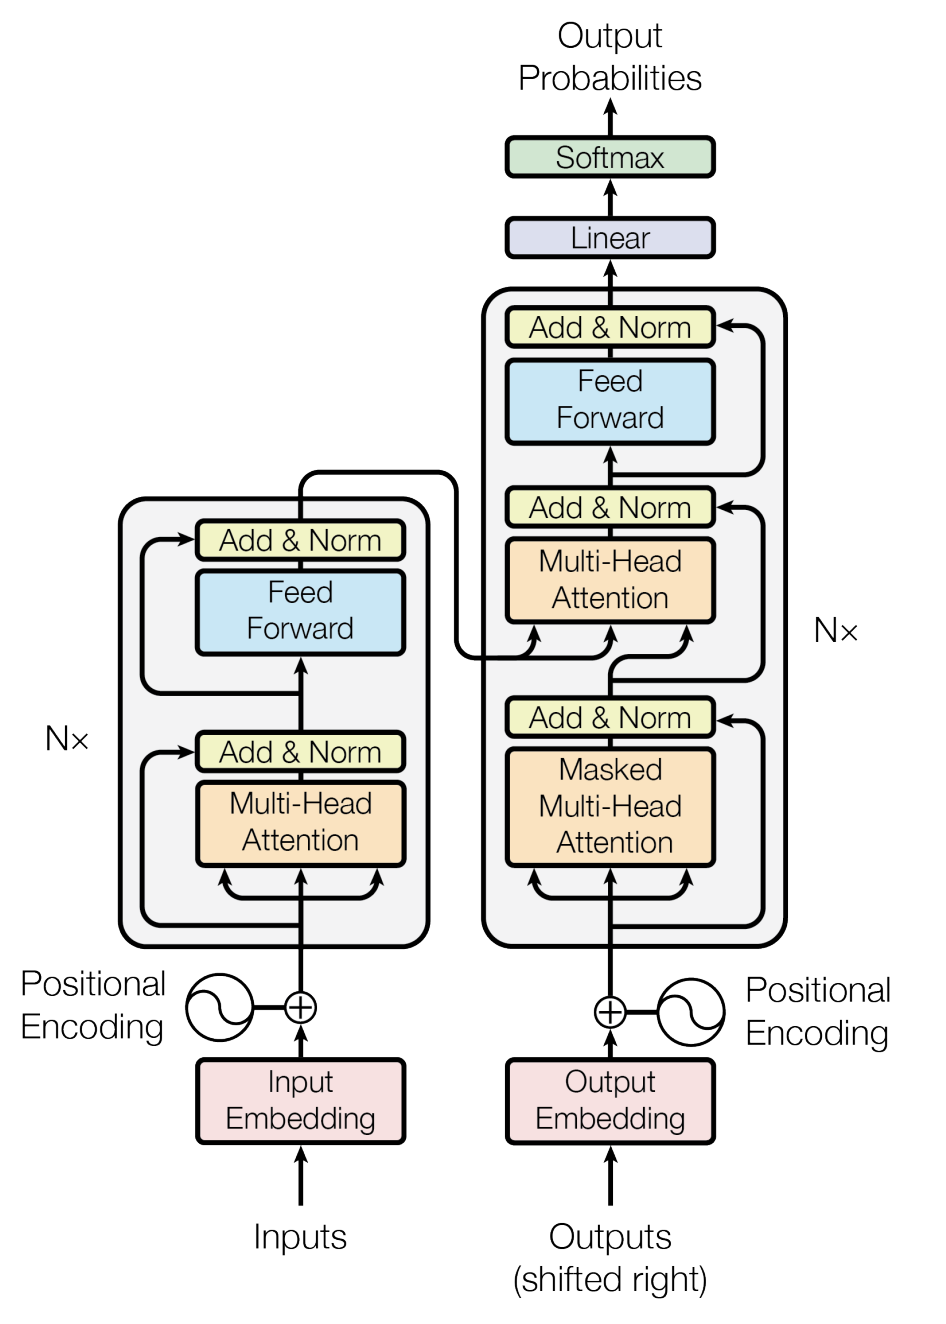
\includegraphics[width=0.5\linewidth]{images/fig/attention.png}
\vspace*{-4mm}
\caption{Architektura Transformera. \cite{attention_2023vaswani} }
% \label{fig:}
\end{figure}

Podczas trenowania dużych modeli językowych wykorzystywane są duże korpusy danych zawierające teksty pochodzące z książek, artykułów, stron internetowych i innych dostępnych dokumentów. Zbiory te obejmowały szeroki wachlarz tematów i stylów pisania. Trening wykorzystywał algorytm wstecznej propagacji błędu (ang. \textit{backpropagation}). Model generuje przewidywania, które są porównywane z rzeczywistymi danymi (np. prawdziwymi słowami w zdaniu). Na tej podstawie obliczany jest błąd, czyli różnica między przewidywaniami, a rzeczywistymi wartościami. Błąd jest następnie propagowany z powrotem przez sieć. Algorytm oblicza, jak bardzo każdy neuron przyczynił się do tego błędu, wykorzystując pochodne funkcji aktywacji. Na podstawie obliczonego błędu i gradientów wag model aktualizuje swoje wagi przy użyciu algorytmu optymalizacji (np. \textit{Stochastic Gradient Descent} lub jego wariantów). Celem jest minimalizacja błędu w kolejnych iteracjach.

Powyższe opisy dotyczą algorytmów używanych w etapie \textit{pre-treningu}, gdzie model uczy się określonych wzorców językowych. Po tym etapie następuje \textit{fine-tuning}, który doszkala model, by dostosować go do konkretnych zadań przez dostarczenie mu bardziej specjalistycznych danych. Ten dwuetapowy proces pozwala na tworzenie bardzo wszechstronnych modeli, które mogą być łatwo dostosowane do różnych aplikacji, takich jak tłumaczenie maszynowe, odpowiadanie na pytania czy analiza sentymentu.

Sukces dużych modeli językowych możliwy jest przez zdolność do uogólniania wiedzy zdobytej podczas pre-treningu i jej zastosowania do nowych, nieznanych wcześniej zadań. Model może generować spójne i trafne teksty jednocześnie bez specjalistycznego procesu szkolenia.

\subsubsection{LLM Chains: koncepcja i przykłady zastosowania}
Mimo, że rozwój modeli językowych pozwolił na wykorzystanie ich do skomplikowanych zadań, nadal problem stanowi zachowanie kontekstu w długich tekstach. Rozwiązaniem tego problemu jest zastosowanie LLM Chains, czyli koncepcji, która realizuje złożone zadania przez podział na mniejsze etapy. Każdy z etapów obsługiwany jest przez odpowiednio przystosowany LLM. To podejście pozwala na zwiększenie precyzji i skuteczności przetwarzania złożonych zapytań. \cite{llm_chains}

LLM Chains może mieć różną postać, w dużej mierze zależną od zastosowania. Jedną z najprostszych technik jest \textbf{Stuffing Chain}, polegający na dwóch krokach:
\begin{enumerate}
    \item W pierwszym kroku gromadzimy wszystkie cytaty oraz fragmenty dokumentów w jednym prompcie, których jest przesyłany do LLM. 
    \item W drugim kroku fragmenty są analizowane, a na ich podstawie tworzona jest ostateczna odpowiedź. 
\end{enumerate}

Inną popularną metodą LLM Chains jest \textbf{Map-Reduce Chain}, która podobna jest do rozproszonego przetwarzania danych. Metoda ta polega na:
\begin{enumerate}
    \item Krok pierwszy: wstępne przetworzeniu każdego fragmentu dokumentów w LLM.
    \item Krok drugi: Wyniki każdego z przetwarzań scalane są w jedną odpowiedź.
\end{enumerate}

Zupełnie inny sposób działania ma metoda \textbf{Refine Chain}. Dane w tej metodzie przetwarzane są sekwencyjnie.
\begin{enumerate}
    \item Krok pierwszy: przeanalizowanie pierwszego źródła oraz stworzenie wstępnej odpowiedzi.
    \item Krok drugi oraz każdy następny: przeanalizowanie kolejnego źródła i ewentualna korekta odpowiedzi.
\end{enumerate}

\textbf{Router (lub Conditional) Chain} to metoda, która zapewnia elastyczność i dopasowanie do zadania. Minusem jest posiadanie scenariusza dla każdego typu promptu oraz posiadanie dobrego klasyfikatora pytań. Metoda ta składa się z następujących kroków: 
\begin{enumerate}
    \item Krok pierwszy: wybór metody w zależności od zadania zawartego w prompcie.
    \item Krok drugi: wykonanie zadania, zgodnie ze ścieżka przypisaną do metody.
\end{enumerate}

Ostatnią z głównych klasycznych typów LLM Chains jest \textbf{Iterative / Self-Ask Chain}, czyli metoda, gdzie model sam generuje pytania pomocnicze i generuje odpowiedź krok po kroku. 

W powyższym omówiliśmy tylko najbardziej klasyczne typy LLM Chains. Poszczególne składowe kroków, mogą się różnić w zależności od zadania oraz możliwości. LLM Chains mogą być stosowane między innymi w systemach rekomendacji. Przykładem może być platforma e-commerce, gdzie pierwszy model analizuje historię zakupów i zachowania użytkownika, drugi model identyfikuje podobne produkty lub usługi, a trzeci model generuje spersonalizowane rekomendacje. Dzięki zastosowaniu łańcucha modeli, platforma może zapewnić bardziej trafne i spersonalizowane sugestie dla użytkowników. 

Koncepcja LLM chains jest nie tylko potężnym narzędziem w kontekście przetwarzania języka naturalnego, ale także elastycznym podejściem, które może być dostosowane do różnych dziedzin i zastosowań. Dzięki możliwości segmentacji złożonych zadań na mniejsze, wyspecjalizowane etapy, LLM chains umożliwiają bardziej efektywne i precyzyjne przetwarzanie danych, co otwiera nowe możliwości dla zaawansowanych aplikacji w różnych sektorach.

\subsection{RAG}

\subsubsection{Definicja i koncepcja RAG}

\textbf{Retrieval Augmented Generation (RAG)} to zaawansowana technika przetwarzania języka naturalnego, która łączy dwa kluczowe komponenty: wyszukiwanie informacji (\textit{retrieval}) i generowanie tekstu (\textit{generation}). Celem RAG jest poprawa jakości generowanych odpowiedzi poprzez wykorzystanie zewnętrznych źródeł wiedzy, co pozwala na bardziej trafne i kontekstowe odpowiedzi na pytania użytkowników. Koncepcja ta stanowi istotny postęp w dziedzinie QA systems (systemy pytanie - odpowiedź) oraz aplikacji NLP, gdzie istotne jest nie tylko rozumienie pytania, ale także dostarczenie precyzyjnych informacji opartych na dużych bazach danych. \cite{rag}

W klasycznym podejściu do generowania tekstu, modele językowe bazują wyłącznie na wewnętrznej wiedzy zdobytej podczas treningu na dużych zbiorach danych. Modele takie jak Chat GPT od OpenAI mają ograniczenia związane z ich statycznym charakterem. Nie są w stanie dynamicznie uwzględniać nowych informacji, które pojawiły się po zakończeniu treningu. Ten problem można rozwiązać przez zastosowanie RAG, który integruje komponent wyszukiwania informacji, umożliwiając modelowi dostęp do najnowszych danych z zewnętrznych źródeł, takich jak bazy danych, artykuły, dokumenty czy strony internetowe.

Problem stateczności modelu został rozwiązany w systemie Chat GPT-4 oraz Chat GPT-5, które to mają dostęp do tworzenia zapytań w internecie. \cite{8_aa} W dokumentacji OpenAI nie jest do końca stwierdzone jawnie, że Chat GPT-4 lub GPT-5 korzysta z RAG-a, ale zawarta jest informacja, że Chat GPT-4 może korzystać z systemów lub narzędzi, wspomagających tworzenie odpowiedzi. \cite{9_aa}

Dzięki zdolności do łączenia statycznej wiedzy modeli językowych z dynamicznymi informacjami z zewnętrznych źródeł, RAG stanowi potężne narzędzie, które znacząco zwiększa efektywność i użyteczność aplikacji NLP.

\subsubsection{Architektura i komponenty RAG}
Architektura \textbf{\textit{Retrieval-Augmented Generation (RAG)}} łączy możliwości dużych modeli językowych z mechanizmami wyszukiwania informacji. W tym rozdziale poruszymy główne elementy architektury RAG oraz sposób, w jaki współpracują one w procesie przetwarzania zapytań. W paradygmacie RAG rozróżniamy 3 możliwe typy architektury: Naive RAG, Advanced RAG oraz Modular RAG.\cite{10_aa} Typu te różnią pod względem budowy. Metoda RAG jest i przewyższa wydajność zwykłych LLM, jednak posiada ograniczenia. Powstanie Advanced RAG i Modular RAG jest odpowiedź na te niedociągnięcia w Naive RAG.

Native RAG jest podstawową architekturą, jej architektura znajduje się na rysunku 2. W pierwszym kroku potrzebujemy \textbf{promptu (input)}, który jest wprowadzony przez użytkownika. User wprowadził prompt z pytaniem, na przykład o niedawne wydarzenie lub najnowszych aktualizacjach informacji w jakiejś dziedzinie. Model miał jednak trening na danych nie posiadających informacji na ten temat. 

W kolejnym kroku następuje \textbf{\textit{indexing}}. Dane najpierw zostają oczyszczone i wyodrębnione z surowych danych, który mogły być przechowywane w różnych formatach. Następuje konwertowanie na jeden wspólny format. Informacje podzielone są na chunki, czyli mniejsze elementy tekstu. Na koniec tego etapu dane zamieniane są w wektory przy wykorzystaniu \textbf{\textit{embeddingu}}. 

Kolejny krok - \textbf{\textit{retrieval}} polega na obliczeniu podobieństwa między wektorami promptu oraz wektorami powstałymi podczas \textbf{\textit{indexingu}}. Ustalone zostają priorytetowe informacje, które mają największe prawdopodobieństwo dopasowania. Informacje te są dodane jako rozszerzony kontekst. 

Ostatni krok  - \textbf{\textit{generation}} to generowanie odpowiedzi na podstawie informacji dostarczonych jako rozszerzony kontekst lub/i wiedzy, na podstawie, której szkolony był model językowy. 

\begin{figure}[H]
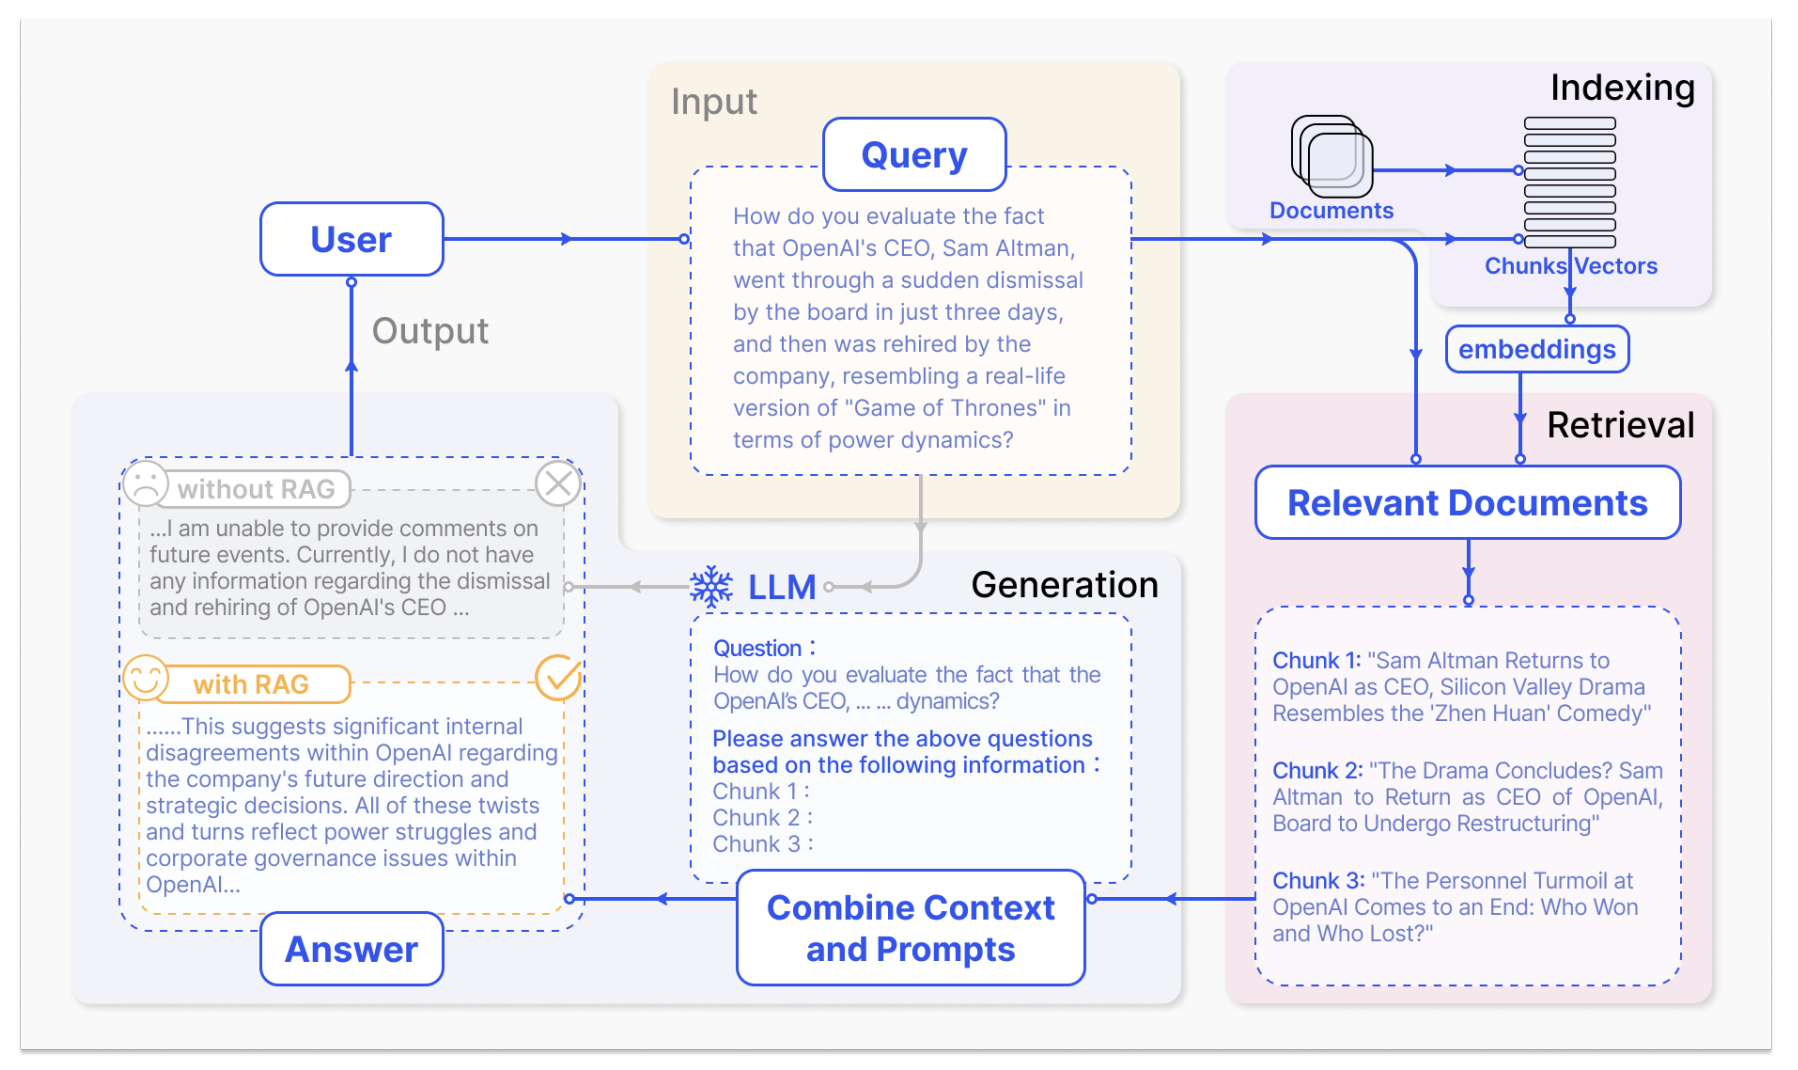
\includegraphics[width=\linewidth]{images/fig/rag.png}
\vspace*{-10mm}
\caption{Przykład procesu RAG zastosowanego do odpowiadania na pytania. Składa się głównie z 3 kroków. \textbf{1) Indexing}: Dokumenty są podzielone na kawałki, zakodowane w wektorach i przechowywane w bazie danych wektorów. \textbf{2) Retrieval}: Pobierz najważniejsze k fragmentów najbardziej odpowiednie dla pytania w oparciu o podobieństwo semantyczne. \textbf{3) Generation}: Wprowadź pierwotne pytanie i pobrane fragmenty razem do LLM, aby wygenerować ostateczną odpowiedź. \cite{10_aa}}
% \label{fig:}
\end{figure}

Naive RAG rozszerza kontekst LLM, dzięki czemu odpowiedzi są trafne lub dostarczają dodatkowych informacji, świeżych aktualizacji wiedzy. Typ ten posiada jednak swoje ograniczenia. Krok \textbf{\textit{retrieval}} ma problem z precyzją co może prowadzić do wyboru nieodpowiednich fragmentów informacji. Dodatkowo może być podatny na halucynacje przez dostarczenie stronniczych informacji. Podczas kroku \textbf{\textit{generation}} mogą pojawiać się problemy z niespójnością oraz powtarzaniem podobnych informacji przez ich duplikaty w odrębnych źródłach. Model LLM może również zbytnio polegać na rozszerzonym kontekście co może prowadzić do parafrazowania źródła bez rozszerzenia, analizowania czy syntezy informacji w nich zawartych.

Wychodząc naprzeciw ograniczeń typu \textbf{\textit{Naive RAG}} powstał typ \textbf{\textit{Advanced RAG}}, który koncentruje się na poprawie jakości wyszukiwanych informacji. Różnice w architekturze pomiędzy Naive RAG oraz Advanced RAG zawarte są na rysunku \ref{fig:advanced_rag}. \textbf{\textit{Advanced RAG}} również składa się z kroku indexing, retrieval oraz generation. Dodatkowo dodane są \textbf{\textit{pre-retrieval}} - poprzedzający proces retrievalu oraz \textbf{\textit{post-retrieval}}, który odbywa się nim. 

\begin{figure}[H]
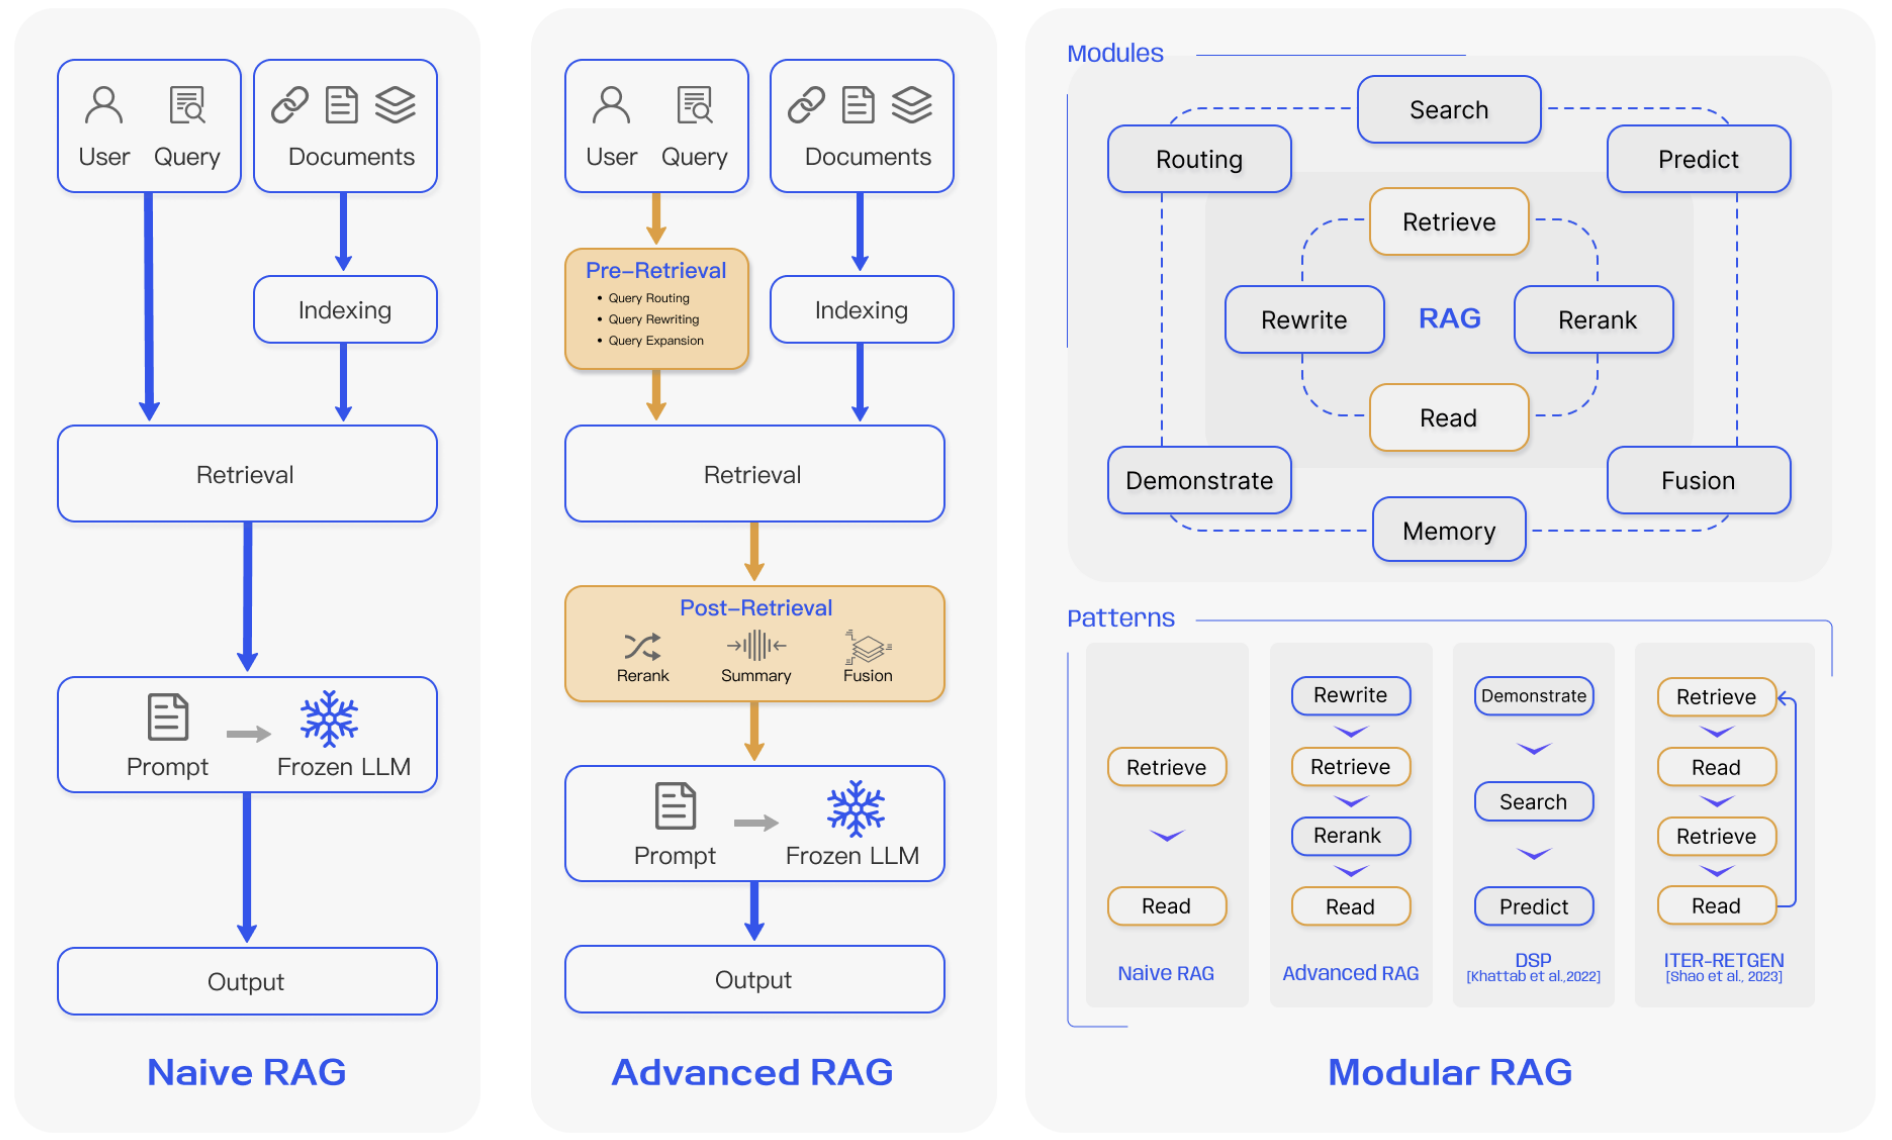
\includegraphics[width=\linewidth]{images/fig/advanced_rag.png}
\vspace*{-10mm}
\caption{Różnice między poszczególnymi typami RAG. Po lewej - Naive RAG składa się głównie z trzech części: indeksowania, wyszukiwania i generowania. (Środek) Advance RAG proponuje wiele strategii optymalizacji dotyczących pobierania przed i po pobraniu, z procesem podobnym do Naive RAG, wciąż po strukturę przypominającą łańcuch. (Po prawej) Modułowy RAG dziedziczy i rozwija się z poprzedniego paradygmatu, wykazując się ogólną większą elastycznością. Widać to w wprowadzenie wielu specyficznych modułów funkcjonalnych i wymiana istniejących modułów. Cały proces nie ogranicza się do wyszukiwania sekwencyjnego i generacja; obejmuje metody takie jak wyszukiwanie iteracyjne i adaptacyjne. \cite{10_aa}}
\label{fig:advanced_rag}
\end{figure}

\textbf{\textit{Pre-retrieval}} kładzie nacisk na poprawę struktury indeksowania oryginalnego zapytania przez na przykład zwiększenie ziarnistości danych, optymalizację struktur indeksów, dodawanie metadanych czy wyszukiwanie mieszane. \textbf{\textit{Post-retrieval}} to efektywne zintegrowanej z zapytaniem. Metody używane na etapie post-retrievalu to powtórny ranking fragmentów, kompresja kontekstu oraz ponowne uszeregowanie pobranych informacji w celu przeniesienia najbardziej istotnych monitów na początek monitu.

Ostatnim typem RAG jest \textbf{\textit{Modular RAG}} wychodzi poza ramy poprzednich dwóch typów, pozwalając na większe dopasowanie rozwiązania pod problem oraz wszechstronność. Architektura Modular RAG to zastosowanie wymiennych komponentów zamiast jednego sztywnego pipeline'u. Modular RAG oddziela poszczególne etapy procesu (pre-retrieval, retrieval, post-retrieval, reasoning, generation, ewaluacja) i pozwala wymieniać je niezależnie. Dodatkowym komponentem w  może być na przykład feedback-loop zapewniająca fact-checking czyli sprawdzenie poprawności danych z źródłami zewnętrznymi.

RAG jest jednym z sposobów optymalizacji odpowiedzi LLM na prompty użytkowników. Na rysunku \ref{fig:modular_rag} przedstawione są inne sposoby wpływania na odpowiedź modelu. Warto zauważyć, że RAG jest, który w korzysta głównie z zewnętrznych źródeł, bez dodatkowego trenowania modelu. RAG może być zastosowany jako pojedyncze narzędzie lub razem z innymi sposobami takimi jak fine-tuning - dodatkowe uczenie modelu pod dane zadanie lub prompt engineering czyli używanie technik pisania promptów w celu optymalizacji odpowiedzi LLM.

\begin{figure}[H]
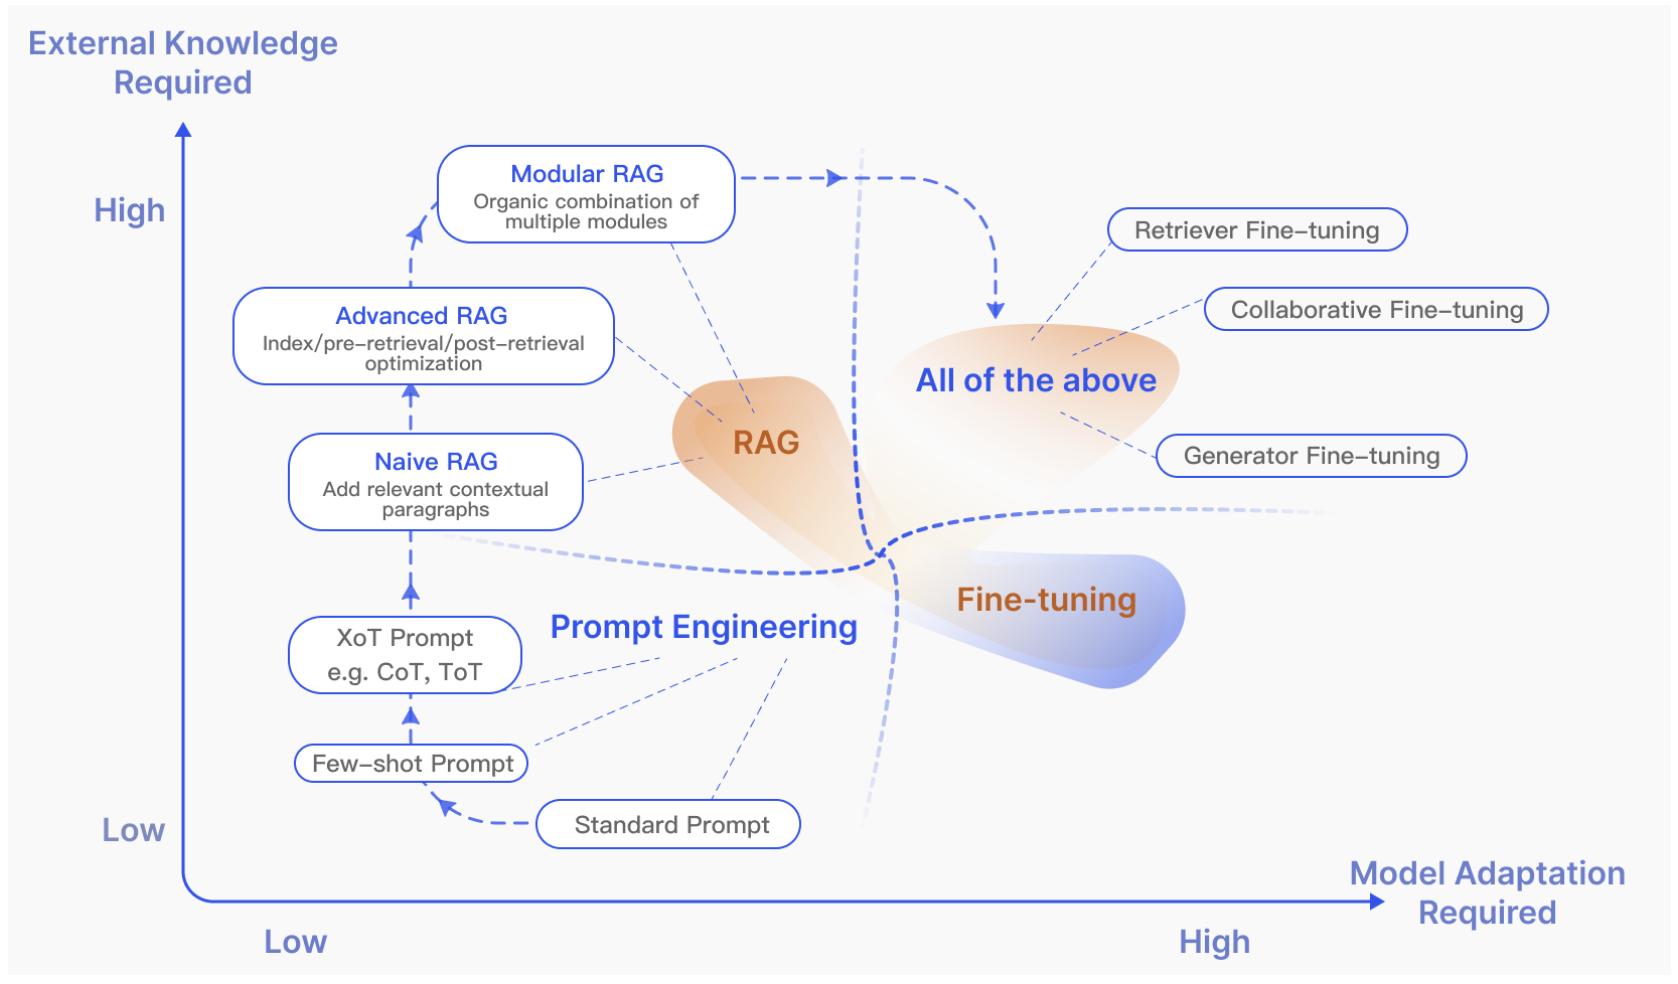
\includegraphics[width=\linewidth]{images/fig/modular_rag.png}
\vspace*{-10mm}
\caption{RAG w porównaniu z innymi metodami optymalizacji modelu w aspektach „Wymagana wiedza zewnętrzna” i „Wymagana adaptacja modelu”. Podpowiedź
Inżynieria wymaga niewielkich modyfikacji modelu i wiedzy zewnętrznej, skupiając się na wykorzystaniu możliwości samych LLM. Dostrajanie, włączone
z drugiej strony wymaga dalszego szkolenia modelu. We wczesnych stadiach RAG (Naive RAG) zapotrzebowanie na modyfikacje modelu jest niskie. Jako badania
się rozwija, Modular RAG stał się bardziej zintegrowany z technikami dostrajania. \cite{10_aa}}
\label{fig:modular_rag}
\end{figure}

Z kolei Dense Passage Retrieval wykorzystuje zaawansowane techniki uczenia maszynowego, aby zakodować zarówno zapytania, jak i dokumenty w przestrzeni wektorowej, co umożliwia bardziej precyzyjne dopasowanie zapytań do dokumentów poprzez obliczanie odległości w tej przestrzeni.

\subsubsection{Zalety i wyzwania związane z RAG}

RAG jest innowacyjnym narzędziem, które pozwala na optymalizację odpowiedzi LLM oraz wpływa na jakość oraz rzetelność informacji zawartych w odpowiedziach.  Jednak Jak każde narzędzie RAG posiada swoje zalety oraz ograniczenia.

Głównymi zaletami RAG jest dostarczanie trafnych informacji i możliwość aktualizowania wiedzy zawartej w modelu. Tradycyjne modele językowe są ograniczone do wiedzy zdobytej podczas treningu, co oznacza, że nie mogą dynamicznie reagować na nowe informacje pojawiające się po zakończeniu procesu treningowego. RAG rozwiązuje ten problem, łącząc generowanie tekstu z dynamicznym wyszukiwaniem informacji. Dzięki temu odpowiedzi generowane przez RAG są bardziej aktualne, precyzyjne i kontekstowe, co jest szczególnie istotne w szybko zmieniających się dziedzinach, takich jak medycyna, technologia czy finanse.

W pracy  Retrieval-Augmented Generation for Large Language Models: A Survey omówione zostały następujące wady oraz zalety pracy z RAG. Głównym pojawiającym się problemem w architekturze jest skalowalność oraz integracja komponentów retrievera i generatora. Proces ten wymaga precyzyjnego dostosowania obu komponentów, aby działały one harmonijnie i efektywnie.

Następne wyzwanie pojawia się na etapie Retrieval napotyka trudności z precyzją i przypominaniem kontekstu, co prowadzi do niespójnych lub nieistotnych fragmentów odpowiedzi. 

Na etapie generation LLM jak w innych rozwiązaniach może generować halucynacje czyli spójne językowo odpowiedzi, które mijają się z prawdą lub są fikcją. Faza ta może mieć również problem z stronniczością w odpowiedzi lub generować kontrowersyjne treści z uwagi na dostarczone źródła co wpływa na rzetelność modelu. 

Na etapie augmentation pojawia się problem integracji wyszukanych informacji, co może skutkować niespójnymi wynikami. Odpowiedzi generowane przez model mogą także zawierać redundancje, czyli powtarzanie tych samych treści w różnych fragmentach odpowiedzi. Nie wpływa to bezpośrednio na rzetelność modelu, jednak obniża użyteczność danych i może wymagać dodatkowej obróbki.

Dodatkowym wyzwaniem jest określenie znaczenia i trafności poszczególnych fragmentów kontekstu oraz zapewnienie spójności stylistycznej i tonalnej całej odpowiedzi. W przypadku bardziej złożonych zapytań pojedyncze wyszukiwanie oparte wyłącznie na oryginalnym pytaniu często okazuje się niewystarczające do uzyskania adekwatnych informacji kontekstowych.

Co więcej, istnieje ryzyko, że modele generujące będą nadmiernie polegać na dostarczonym kontekście, ograniczając się do powtarzania treści zamiast oferować głębszą analizę czy syntezę informacji.

Powyższe wyzwanie mogą być ograniczone poprzez zastosowanie modułu fakt-checkingu lub wykorzystania dodatkowego modułu, który poprawia jakość odpowiedzi.

\subsection{Graph RAG}

\subsubsection{Definicja i koncepcja Graph RAG}

Graph Retrieval Augmented Generation (Graph RAG) to zaawansowane podejście do przetwarzania języka naturalnego, które łączy tradycyjne techniki Retrieval Augmented Generation (RAG) z wykorzystaniem grafów wiedzy (Knowledge Graphs, KG). Podstawową ideą Graph RAG jest wykorzystanie struktury grafu do organizowania i przetwarzania informacji, co pozwala na bardziej złożone i semantycznie bogate reprezentacje danych. Dzięki temu możliwe jest generowanie bardziej precyzyjnych i kontekstowych odpowiedzi na zapytania użytkowników.

\subsubsection{Architektura Graph RAG}

todo


\subsubsection{Zalety Graph RAG w porównaniu do standardowego RAG}

todo


%%% -----------------

%%% Część praktyczna
\section{Część praktyczna}

\subsection{Opis zbioru danych (dane o filmach)}

Do badania zostały wybrane dane o 1000 filmach z bazy IMDB \cite{11_aa}, są to dane ustrukturyzowane i zapisane w pliku csv. Ponieważ w tej pracy rozważamy przypadek pracy z danymi tekstowymi to informacje o filmach zapisujemy do plików tekstowych w przedstawionej poniżej formie:

% \begin{codestyle}[]\\
% Movie name: The Shawshank Redemption\\
% Released year: 1994\\
% Runtime: 142 min\\
% Genres: Drama\\
% Rating: 9.3\\
% Short description: Two imprisoned men bond over a number of years, finding solace and eventual redemption through acts of common decency.\\
% Director: Frank Darabont\\
% Actors: Tim Robbins, Morgan Freeman, Bob Gunton, William Sadler\\
% No of rating votes: 2343110\\
% Gross revenue: 28341469\\
% \end{codestyle}
\begin{codestyle}
Movie name: The Shawshank Redemption
Released year: 1994
Runtime: 142 min
Genres: Drama
Rating: 9.3
Short description: Two imprisoned men bond over a number of years, finding solace and eventual redemption through acts of common decency.
Director: Frank Darabont
Actors: Tim Robbins, Morgan Freeman, Bob Gunton, William Sadler
No of rating votes: 2343110
Gross revenue: 28341469
\end{codestyle}

Dane tekstowe w takim formacie (etykieta: wartość) nadają się do wysłania w zapytaniu do LLM, ponieważ minimalizują możliwość błędnej interpretacji wartości.

Dane te symulują przypadek, gdy przeprowadzony zostanie web scraping (programowe, algorytmiczne odczytywanie informacji ze stron internetowych) danych z serwisów filmowych typu Filmweb, IMDB. Dane w analogiczny sposób można wydobyć z plików pdf, czy nawet filmów (przy czym dla filmów jest to zadanie znacznie bardziej skomplikowane, wymagające dużej mocy obliczeniowej i czasu działania oraz ze względu na proces transkrypcji - bardzo podatne na błędy identyfikacji słów czy wyrażeń). W tej pracy krok ten nie jest wykonywany (a jego wynik jest symulowany w wyżej opisany sposób), ponieważ nie jest on przedmiotem badania w tej pracy i nie jest wymagany do jej realizacji.

Tekst z wybranego zbioru jest w języku angielskim, dlatego też dane te są dalej etykietowane w tym języku i w nim też będą odbywały się zapytania. W związku z tym należy zaznaczyć, że zarówno modele LLM jak i modele wektoryzujące są w znacznej większości trenowane na danych anglojęzycznych co ma znaczący wpływ na jakość i dokładność ich odpowiedzi, wyników. Należy zatem odnotować, że rozważane badania RAG vs Graph RAG są najlepszym wariantem danych wejściowych dla modeli LLM i wektoryzujących.

\subsection{Wybrany LLM}

Do realizacji algorytmów RAG i Graph RAG wybrany został jeden z najbardziej zaawansowanych wielkich modeli językowych w czasie realizacji tej pracy - OpenAI GPT-4.1. Dostępny za darmo z limitem 250 tys. tokenów dziennie, pod warunkiem udzielenia przez użytkownika zgody, by OpenAI miało dostęp do jego zapytań i odpowiedzi LLM.

W toku rozwoju pracy używane też były inne modele (Llama 3, Llama 3.1, Gemma2) z bazy publicznie dostępnych modeli LLM - Ollama - i używane one były na komputerze lokalnie. Niestety dostępny komputer nie był w stanie obsłużyć modeli większych niż 7B (7 miliardów aktywnych parametrów), co sprawiało że odpowiedzi LLM były niewystarczające (np. w przypadku tak trudnego zadania jak napisanie zapytania do bazy Neo4j w języku CYPHER, gdzie owe ‘małe’ modele często tworzyły zapytania nie dające poprawnych odpowiedzi z bazy), co sprawiało że nie są one reprezentatywnym przykładem do przedstawienia w tej pracy. W związku z tym warte odnotowania jest, iż o ile takie modele nie nadają się do tworzenia np. zapytań do bazy, to są wystarczające do stworzenia ostatecznej odpowiedzi, w ostatnim etapie gdzie mamy już pobrane dane na podstawie których LLM ma udzielić odpowiedź (o ile cały dostarczony kontekst zmieści się w maksymalnej liczbie tokenów wejściowych do tego modelu).

\newpage
\begin{python}
from langchain_openai import ChatOpenAI

llama3 = ChatOpenAI(
    api_key = "ollama",
    base_url = "http://host.docker.internal:11434/v1",
    model = "llama3.1", 
    temperature = 0,
)

# You're eligible for free daily usage on traffic shared with OpenAI:
# - up to 250 thousand tokens per day across gpt-4.5-preview, gpt-4.1, gpt-4o, o1 and o3
# - up to 2.5 million tokens per day across gpt-4.1-mini, gpt-4.1-nano, gpt-4o-mini, o1-mini, o3-mini, o4-mini, and codex-mini-latest
gpt4 = ChatOpenAI(
    model = "gpt-4.1", # "gpt-3.5-turbo", "gpt-4o"
    temperature = 0,
    max_tokens = None,
    timeout = None,
    max_retries = 2,
    api_key = OPENAI_API_KEY,
)
\end{python}

Na wybranym kawałku kodu widać, jak zostały stworzone połączenia do modeli GPT-4.1 i Llama 3.1. Ważny jest tutaj parametr temperature, który to kontroluje losowość lub „kreatywność” wyników modelu i przyjmuje wartości z zakresu 0.0 do 1.0. Niższa temperatura skutkuje bardziej przewidywalnymi i ukierunkowanymi reakcjami, podczas gdy wyższa temperatura sprzyja bardziej zróżnicowanym i potencjalnie kreatywnym wynikom. Ponieważ w tej pracy zależy nam, żeby model dokładnie wykonywał instrukcje i korzystał z wiedzy którą dostarczamy w RAG lub Graph RAG, parametr ten został ustawiony na wartość 0.

\subsection{Rozwiązanie RAG}
\textcolor{red}{\textit{? Opis ogólny dodać ?  co robimy, jak i dlaczego - bez kodu, nietechnicznie}}

\subsubsection{Wektoryzowanie danych tekstowych}
\textcolor{red}{\textit{! Opis ogólny dodać ?  co robimy, jak i dlaczego - bez kodu, nietechnicznie}}

\subsubsubsection{Metoda wektoryzacji tekstu}

Wybranym modelem do wektoryzacji tekstu został text-embedding-3-small\cite{te3s} autorstwa OpenAI, który generuje embeddingi w przestrzeni 1536 wymiarowej.
\textcolor{red}{Embeddingi to numeryczne reprezentacje tekstu w postaci wielowymiarowych wektorów, które pozwalają obliczyć podobieństwo dwóch tekstów. Wektory te są użyteczne w zadaniach związanych z przeszukiwaniem, klastrowaniem, rekomendacjami oraz klasyfikowaniem.}
(Jest on) \textcolor{red}{Wybrany model jest} 
oferowany jako usługa SaaS (Software as a Service) i jest jednym z najlepszych narzędzi tego typu dostępnych na rynku, i jest udostępniany w przystępnej cenie. Istnieje również bardziej zaawansowany model text-embedding-3-large\cite{te3l}, jednak jest on 7 razy droższy co zaważyło o decyzji wybrania modelu small. Zadaniem modelu jest wygenerowanie embeddingów, które zostaną zapisane w bazie wektorowej Pinecone, dzięki czemu będzie później możliwy do przeprowadzenia proces wyszukiwania tekstów (retrieval) powiązanych z pytaniem użytkownika.

Istnieją również inne modele wektoryzujące m.in. $\text{all-MiniLM-L6-v2}$\cite{miniLM}, $\text{nomic-embed-text-v1}$\cite{nomic} - natomiast ich wyniki są mniej dokładne on wybranego, zwłaszcza w kluczowej dla tej pracy operacji znajdowania powiązanych tekstów (retrieval). 

\subsubsubsection{Wektorowa baza danych - Pinecone}

W pracy wykorzystujemy wektorową bazę danych Pinecone, ponieważ zapewnia ona dodatkowe funkcjonalności, z których korzystamy. U podstaw baza ta przechowywuje embeddingi tak jak na przykład biblioteka FAISS (Facebook AI Similarity Search)\cite{faiss}, dzięki czemu zwektoryzowane dane możemy zapisać i później wysyłać zapytania o dane podobne do pytania użytkownika (retrieval i similarity search). Ta podstawowa funkcjonalność zapewnia nam możliwość realizacji RAG w najprostszej postaci, w tej pracy nazwanej RAG v1. Natomiast dodatkowe funkcjonalności, których nie zapewnia FAISS, to przechowywanie i możliwość filtrowania po dodatkowych danych (metadanych) \cite{pinecone:metatdata}, które zapisujemy razem z embeddingiem, dzięki czemu jesteśmy w stanie wykonać bardziej zaawansowany RAG, u nas nazwany RAG v2. Poza tym Pinecone zapewnia znacznie więcej korzyści, takich jak zarządzanie dostępem, integrację z usługami firm trzecich, skalowalność przy znacznym rozbudowaniu i obciążeniu bazy, podpodział danych na przestrzenie nazwane (ang. namespaces), jednak te i inne zalety tego rozwiązania nie są wykorzystywane i prezentowane w tej pracy, jako że nie są istotne w realizacji rozważanych implementacji RAG. Wspominamy o nich ponieważ warto odnotować że są to cechy pożądane w komercyjnej realizacji RAG, gdzie poziom skomplikowania drastycznie rośnie i trzeba zadbać o bezpieczeństwo danych i stabilność rozwiązania dla klientów. 

\subsubsubsection{Implementacja i narzędzia wykorzystywane do wektoryzacji}













% \newpage\null
\blankpage
% \newpage
\subsection{Wnioski i analiza wyników}

\subsubsection{Opis metodologii badawczej}

W celu porównania zaproponowanych w tej pracy rozwiązań RAG i Graph RAG, przygotowaliśmy 100 pytań \textbf{[załącznik / przypis do pliku z pytaniami?]} o filmy, reżyserów, aktorów, statystyki, itp, o różnym poziomie skomplikowania, od prostszych pytań o fakty (np. “Kto wyreżyserował Ojca Chrzestnego?”) do takich wymagających pewnego rozumowania (np. “Podaj listę filmów, które mogą się spodobać entuzjaście Incepcji.”).

Następnie na każde z tych pytań ręcznie odnajdujemy poprawną odpowiedź (co wymagało wiele wysiłku i trwało wiele godzin), by stworzyć źródło prawdy, do którego to będziemy porównywać odpowiedzi przedstawionych wcześniej rozwiązań. Porównań tych jednak nie musimy znów robić ręcznie, ale możemy wykorzystać przedstawiane wcześniej embeddingi, by zwektoryzować poprawne odpowiedzi i wykorzystując podobieństwo kosinusowe, porównać je z również zwektoryzowanymi odpowiedziami algorytmów Graph RAG i RAG, dzięki czemu uzyskamy skwantyzowane, numeryczne wyniki, jak podobna jest odpowiedź modelu do oczekiwanej.

Dodatkowo każdą odpowiedź można porównać do oczekiwanej wysyłając obie w zapytaniu do LLM, z instrukcją by ocenił czy odpowiedź zawiera oczekiwane informacje. W takiej metodzie sprawdzenia tych odpowiedzi staramy się wychwycić fakty, czy odpowiedź dostarcza wiedzy której oczekiwaliśmy, a pomijamy samą semantykę i formę budowania zdań w odpowiedzi modelu.

\subsubsection{Porównanie i analiza wyników Graph RAG z RAG v1 i RAG v2}

Zgodnie z oczekiwaniami Graph RAG znacznie częściej uzyskuje wynik podobieństwa do oczekiwanej odpowiedzi wyższy niż RAG v1 i RAG v2 razem, co prezentuje tabela \ref{tab:1}.

\begin{table}[H]
\centering
\begin{tabular}{|c|c|c|}
  \hline 
    \multicolumn{3}{|c|} {Wyższy wynik podobieństwa} \\
  \hline 
    Graph RAG & RAG v2 & RAG v1 \\
  \hline
    78 & 15 & 13 \\
  \hline
\end{tabular} 
\caption{Liczba odpowiedzi dla których metoda uzyskała wyższy wynik niż pozostałe}
\label{tab:1}
\end{table}

Poza samą ilością lepiej ocenionych odpowiedzi, należy również zwrócić uwagę na samą ich jakość, ponieważ mimo iż jedna metoda uzyskała wynik wyższy niż pozostałe nie oznacza to, że jest to odpowiedź poprawna czy chociaż zadowalająca. Dobrze obrazuje to tabela \ref{tab:2}, gdzie widzimy jasno, iż średnio Graph RAG generuje znacznie celniejsze odpowiedzi niż metody RAG v1 i v2.

\begin{table}[H]
\centering
\begin{tabular}{|c|c|c|}
  \hline 
    \multicolumn{3}{|c|} {Średni wynik podobieństwa} \\
  \hline 
    Graph RAG & RAG v2 & RAG v1 \\
  \hline
    0,754 & 0,577 & 0,568 \\
  \hline
\end{tabular} 
\caption{Średni wynik podobieństwa do odpowiedzi oczekiwanej}
\label{tab:2}
\end{table}

Na korzyść Graph RAG przemawia również mediana wyników, przedstawiona w poniższej tabeli, która jest znacznie wyższa od tych prezentowanych przez RAG v1 i v2, ale co ważniejsze, jest również znacznie wyższa od swojej średniej. Z tej obserwacji wynika, że odpowiedzi Graph RAG są na ogół jeszcze lepsze niż wynika to ze średniej, a jednocześnie skłania nas do postawienia hipotezy, iż czasem udziela odpowiedzi o bardzo niskim wyniku.

\begin{table}[H]
\centering
\begin{tabular}{|c|c|c|}
  \hline 
    \multicolumn{3}{|c|} {Mediana} \\
  \hline 
    Graph RAG & RAG v2 & RAG v1 \\
  \hline
    0,831 & 0,610 & 0,598 \\
  \hline
\end{tabular} 
\caption{Mediana wyników podobieństwa do odpowiedzi oczekiwanej}
\label{tab:3}
\end{table}

W celu sprawdzenia tej hipotezy opracowujemy przedstawiony na rysunku \ref{fig:box_plot} wykres pudełkowy. Wyniki uzyskane w eksperymencie we wszystkich trzech metodach charakteryzują się skośnością ujemną. Oznacza to, że rozkład odpowiedzi nie jest symetryczny, lecz przesunięty w stronę wartości wyższych (bliższych 1). Innymi słowy, większość uzyskanych wyników koncentruje się w prawej części przedziału [0, 1], podczas gdy lewy ogon rozkładu (w kierunku wartości bliskich 0) jest wydłużony. Taki kształt rozkładu wskazuje, że modele częściej generują odpowiedzi o stosunkowo wysokich wartościach, natomiast rzadziej – choć nadal istotnie – pojawiają się wyniki znacznie niższe, które powodują odchylenie całego rozkładu w lewą stronę.

\begin{figure}[H]
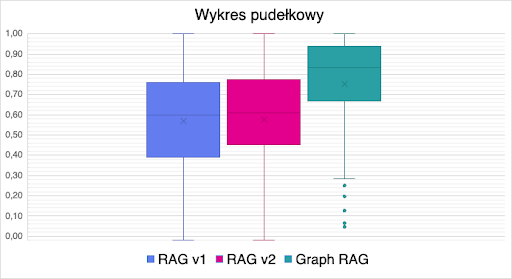
\includegraphics[width=\linewidth]{images/fig/box_plot.png}
\vspace*{-8mm}
\caption{Wykres pudełkowy wyników Graph RAG, RAG v1, RAG v2}
\label{fig:box_plot}
\end{figure}

Największą skośność można zaobserwować w GraphRAG. Metoda ta ma odpowiedzi z największą zgodnością, jednocześnie kilka odpowiedzi miało znaczące gorsze odpowiedzi od pozostałych.







%%% tabela wzorcowa begin
% \begin{table}[H]
% \centering
% \begin{tabular}{|c|c|c|}
%   \hline 
%     \multicolumn{3}{|c|} {title} \\
%   \hline 
%     Graph RAG & RAG v2 & RAG v1 \\
%   \hline
%     0 & 0 & 0 \\
%   \hline
% \end{tabular} 
% \caption{Podpis do tabeli}
% \label{tab:X}
% \end{table}
%%% tabela wzorcowa end

%%% ----------------
\newpage
\clearpage\newpage

%%% Spis rysunków
\listoffigures
\newpage

%%% Bibliografia
\printbibliography{}

%%% Załączniki ?
% https://tex.stackexchange.com/questions/226481/appendix-section-title 


\end{document}